\setstretch{1.2}%řádkování
\hspace{1 cm}
Po spuštění aplikace se otevře dotazové okno, kde je nutné povolit přístup k poloze zařízení (z důvodu že knihovna pro práci s Bluetooth vyžaduje přístup k poloze). Následně se otevře samotná aplikace. Základní grafické rozhraní obsahuje název a stručný popis aplikace, odkaz na GitHub se zdrojovým kódem aplikace a dvě tlačítka - \textbf{1.} připojení zařízení přes Bluetooth, které po rozkliknutí otevře nastavení Bluetooth a zobrazí okolní zařízení, ke kterým se lze připojit, po připojení aplikace zobrazuje název připojeného zařízení; \textbf{2.} export souborů z SD karty zařízení (Arduina), po rozkliknutí tlačítka exportu se zobrazí řádky s názvy souborů uložených na SD kartě připojeného zařízení a k nim přilehlá 3 tlačítka - náhled, stažení a sdílení souboru. Vzhledem k tomu, že se nepodařilo vyřešit problémy s připojováním k Bluetooth zařízení v aplikaci, tak slouží aplikace nainstalovaná pomocí instalačního souboru jako pouhé demo. Na aplikaci je v plánu dále pracovat a další změny budou dostupní na GitHubu.

\begin{figure}[H]
    \centering
    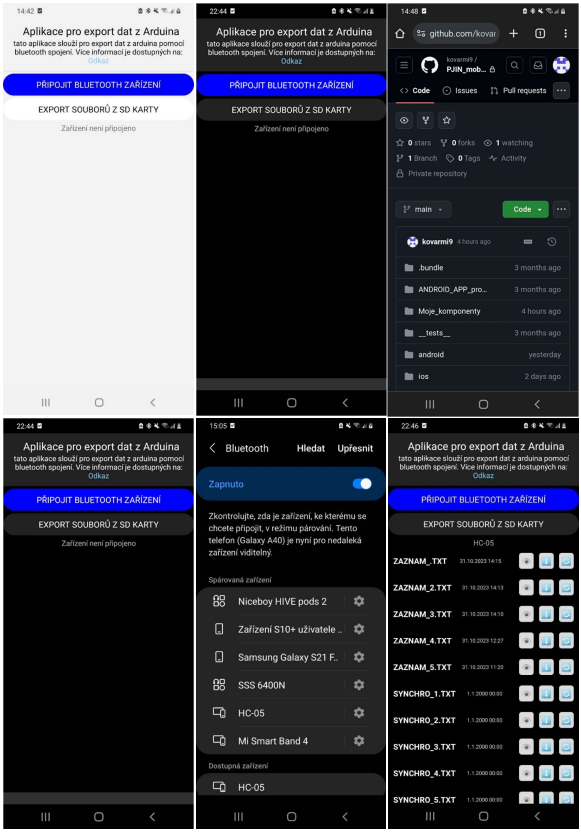
\includegraphics[width=0.5\textwidth]{images/navod_pouzivani.png}
    \caption{Ukázka aplikace}
\end{figure}